\chapter{Sprint 02: 13. Jan, 2015}

\textbf{Sprint beginn:} 10.12.2015
\nextline
\textbf{Sprint ende:} 13.01.2016

\begin{tabular}{|l|l|l|l|l|l|}
            & Datumn        & Name            & \multicolumn{3}{l}{Unterschrift} \\ \hline
Erstellt    & 12. Jan, 2016 & Daniel Melichar & \multicolumn{3}{l}{}             \\ \hline
Geprüft     & 13. Jan, 2016 &                 & \multicolumn{3}{l}{}             \\ \hline
Freigegeben &               &                 & \multicolumn{3}{l}{}            
\end{tabular}

\subsection{Burndownchart}
%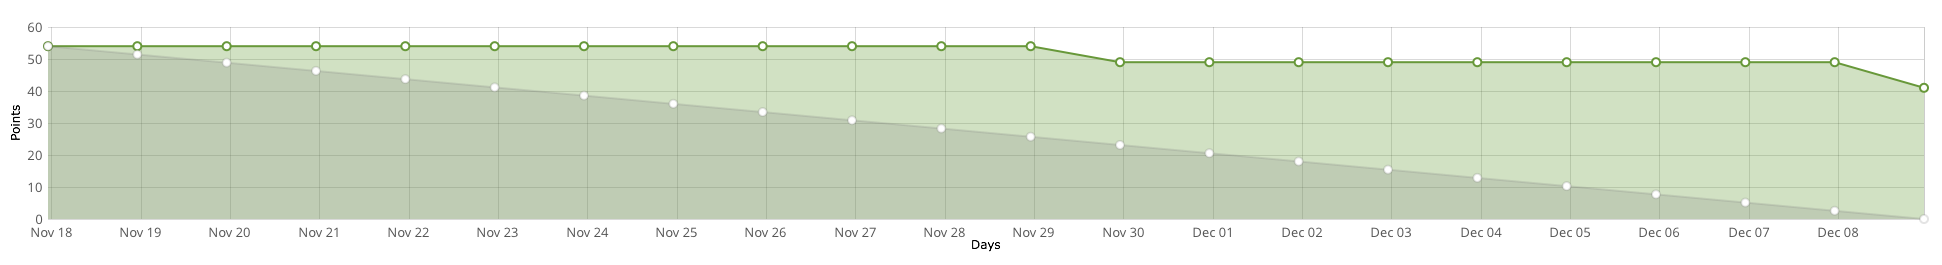
\includegraphics[scale=0.2, ]{images/sprint01-burndown.png}

\subsection{User Stories}
\resizebox{\columnwidth}{!}{%
\begin{tabular}{|l|l|l|l|l|l|}
\hline
\textbf{\#} & \textbf{User Story}                                                                                                                                                                                                                                                                                                                                                                                                                         & \textbf{Story points} & \textbf{Verantwortung} & \textbf{Akzeptanz} & \textbf{Kommentar} \\ \hline
\hline
187 & \begin{tabular}[c]{@{}l@{}}Design der Web-App\\ \\ Als User möchte ich eine anspruchsvolle und einfach zu bedienende Webapplikation haben,\\ damit ich retrospektiv meine Fahrten anschauen kann\\ \\ Akzeptanzkriterien:\\ - Einfach zu bedienen\\ - Übersichtliche Gliederung\\ - Ordnung änderbar\end{tabular} & 8 & Daniel &  &  \\ \hline
185 & \begin{tabular}[c]{@{}l@{}}Akku für Car-PC\\ \\ Als Entwickler möchte ich den Car-PC mit einem Akku ausstatten, damit die\\ gesammelten Daten im Falle eines abrupten\\ Stromausfalles konsistent gehalten werden können\\ \\ Akzeptanzkriterien:\\ - Akku vorhanden\\ - Car-PC für bestimmte Zeit ohne Stromanschluss lauffähig\end{tabular} & 8 & Tobi &  &  \\ \hline
184 & Als Entwickler möchte ich mithilfe eines Car-PCs die Temperatur des Cockpits ermitteln können & 8 & Tobi &  &  \\ \hline
12 & \begin{tabular}[c]{@{}l@{}}Feedback: Statistik der Fahrt\\ \\ Als User möchte ich bei Fahrtende eine Statistik angezeigt bekommen, weil ich\\ gerne wissen würde wie schnell ich gefahren bin, etc.\\ \\ AKZEPTANZKRITERIEN\\ - Statistik nur nach dem Fahrtende\end{tabular} & 3 & Fitim &  &  \\ \hline
14 & \begin{tabular}[c]{@{}l@{}}Gangvorschlag: Gang Genauigkeit\\ \\ Als User möchte ich dass der vorgeschlagene Gang möglichst akurat für mein Fahrzeug kraftstoffsparend berechent wird\\ weil die Applikation mir dabei als Hilfe dienen soll und mir daher bessere Ergebnisse liefern\\ soll als ich eigenständig schaffen würde\end{tabular} & 13 & Raphael &  &  \\ \hline
156 & \begin{tabular}[c]{@{}l@{}}Graph-Design für Handy-App\\ \\ Erstellung der Smarphonefunktion, die die aufbereiteten Daten anzeigt.Mit Mock-Objekten\\ wird der sleep (oder Thread) miteinbezogen, ansonsten wird ein Zeit-Parameter erwartet\end{tabular} & 8 & Bozzy &  &  \\ \hline
15 & \begin{tabular}[c]{@{}l@{}}Datenspeicherung der Sensoren\\ \\ Als Entwickler möchte ich eine Datenbank zum handling der Sensordaten erstellen weil\\ fast jedes Features die aufbereiteten Daten benötigt.\\ \\ Akzeptanzkriterien: \\ - Datenschema auf andere DBMS übertragbar\\ - Neue Sensoren können in die DB speichern\\ - Sensordaten wurden gefiltert\end{tabular} & 8 & Daniel &  &  \\ \hline
6 & \begin{tabular}[c]{@{}l@{}}Sicherung der Sensordaten\\ \\ Als Admin möchte ich einen Datenbank dump \\erstellen können weil ich die Daten damit\\ zu einem späteren Zeitpunkt wieder einfügen kann, bzw. auf einen anderen migrieren.\\ \\ Akzeptanzkriterien: \\ - Sicherung von spezifischen bzw. allen Daten\\ - Sensordaten verschlüsselt\\ - Sensordaten einfach auf (anderes) System migrierbar\end{tabular} & 3 & Daniel &  &  \\ \hline
181 & \begin{tabular}[c]{@{}l@{}}Beschleunigungssensor\\ \\ Als Entwickler möchte ich mithilfe eines Car-PCs die Beschlunigung meines KFZ ermitteln können\\ \\ Akzeptanzkriterien:\\ - Beschleunigungssensor vorhanden\\ - Sensordaten werden in .json File gespeichert\end{tabular} & 8 & Tobi &  &  \\ \hline
8 & \begin{tabular}[c]{@{}l@{}}Kammscher Kreis (Handy)\\ \\ Als User möchte ich mittels eines Buttons einen Kammschen Kreis am Ende der aktuellen\\ Fahrt betrachten können, da ich\\ somit die Beschleunigungskräfte meiner Fahrt betrachten kann\\ \\ Akzeptanzkriterien:\\ Wohlfühlbereich angezeigt\\ Modi auswählbar\end{tabular} & 8 & Fitim &  &  \\ \hline
1 & \begin{tabular}[c]{@{}l@{}}Front- und Querbeschleunigung (Handy)\\ \\ Als User möchte ich eine Visualisierung der front und quer Beschleunigungskräfte sehen, da ich daraus\\ mein aktuelles Fahrverhalten sehen kann.\\ \\ Akzeptanzkriterium: \\ Maximaldauer der Aktualisierung 1sek\\ Chart beschriftet und gut ersichtlich (x,y,z Achse, titel)\\ Vereinbarten Design einhalten (Farbe, Schrift etc)\end{tabular} & 5 & Fitim &  &  \\ \hline
4 & \begin{tabular}[c]{@{}l@{}}Ladebalken\\ \\ Als User möchte ich möglichst von den Wartezeiten abgelenkt werden, damit das nicht\\ so lange wirktLadebalken, Ladeanimation\\ \\ AKZEPTANZKRITERIEN:\\ Verständliche Darstellung des Status\\ Simple Visualisierung\\ (Rotierendes Icon)\end{tabular} & 5 & Bozzy &  &  \\ \hline
23 & \begin{tabular}[c]{@{}l@{}}Gangvorschlag: Gangwechsel Erkennung\\ \\ Als User möchte ich dass ein umgesetzter Gangvorschlag auch als Gangwechsel\\ erkannt wird weil ich während der Fahrt möglichst wenig eigenhändigen Input in der App liefern möchte\end{tabular} & 13 & Raphael &  &  \\ \hline

\end{tabular}
}